\chapter{Verifiche Normativa}

Dopo aver tracciato i profili è necessario che tutti i valori soddisfino i limiti della normativa. OpenRoads ci permette di effettuare queste verifiche attraverso il comando Geometry/Italian checks/Horizontal vertical checks.

\begin{figure}[H]
	\centering
	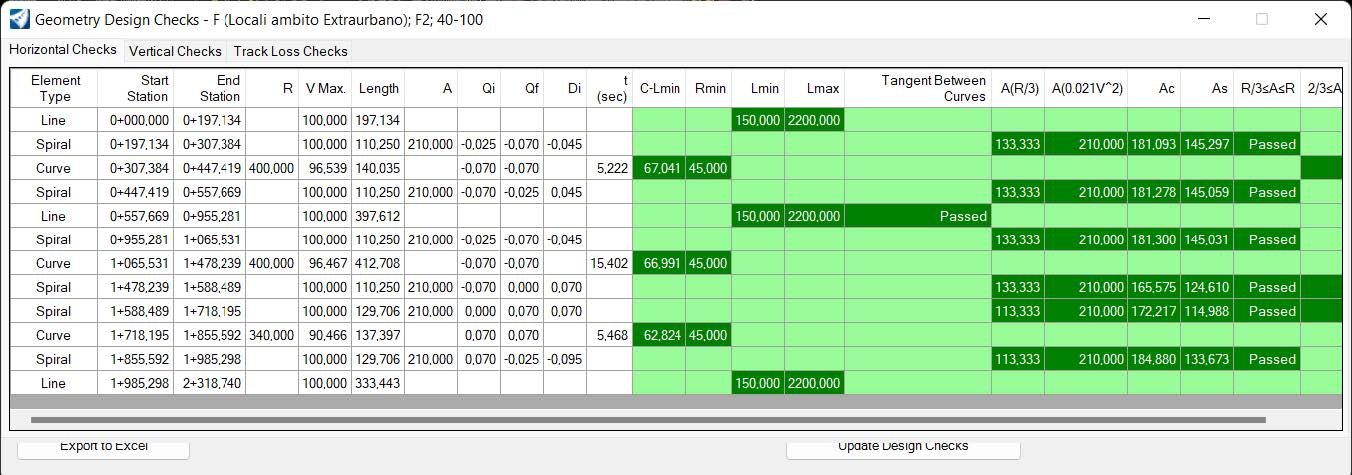
\includegraphics[width=\linewidth]{Figures/Horizontal checks}
	\captionof{figure}{Horizontal checks, Planimetrico}
    \label{fig:Horizontal checks}
\end{figure}

\begin{figure}[H]
	\centering
	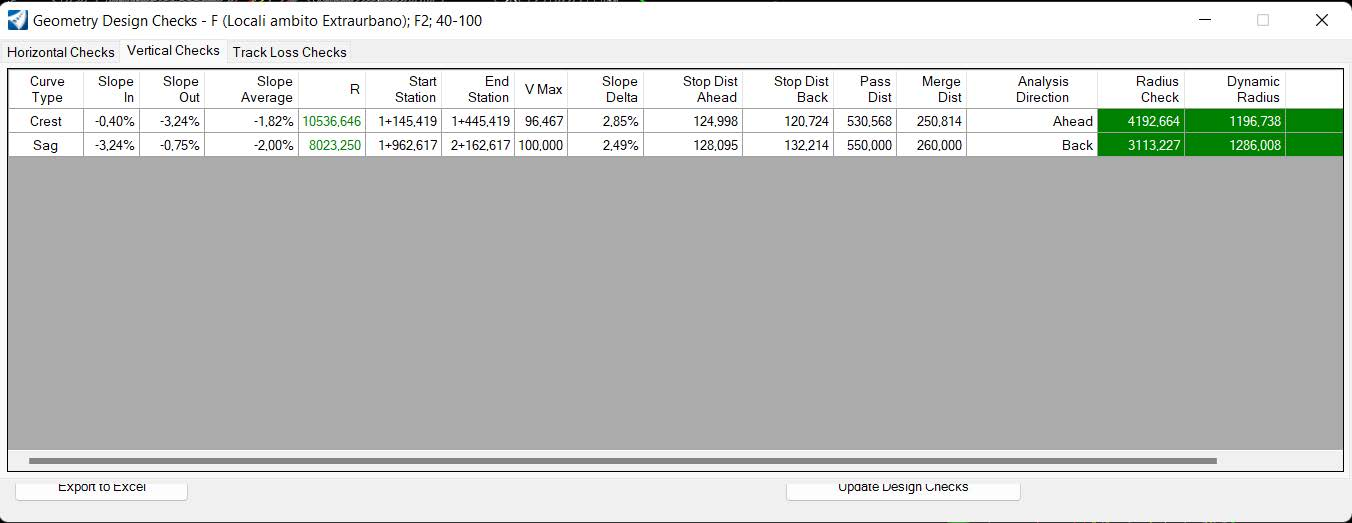
\includegraphics[width=\linewidth]{Figures/Vertical checks}
	\captionof{figure}{Vertical checks, Altimetrico}
    \label{fig:Vertical checks}
\end{figure}

\begin{figure}[H]
	\centering
	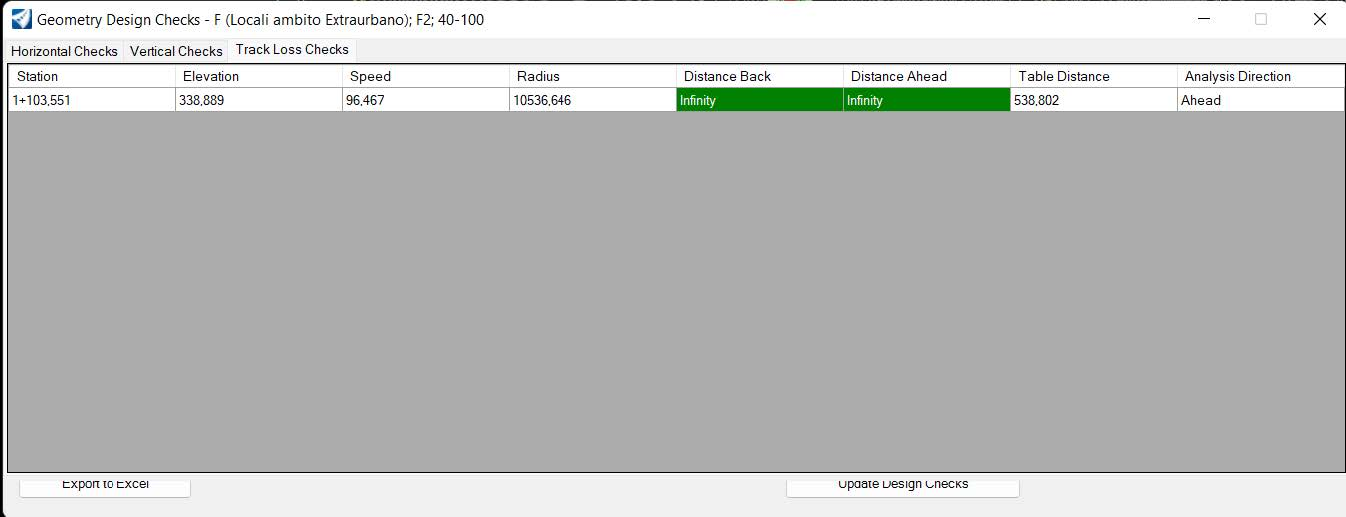
\includegraphics[width=\linewidth]{Figures/Track Loss Checks}
	\captionof{figure}{Track Loss Checks, Perdita di tracciato}
    \label{fig:Track Loss Checks}
\end{figure}

\begin{figure}[H]
	\centering
	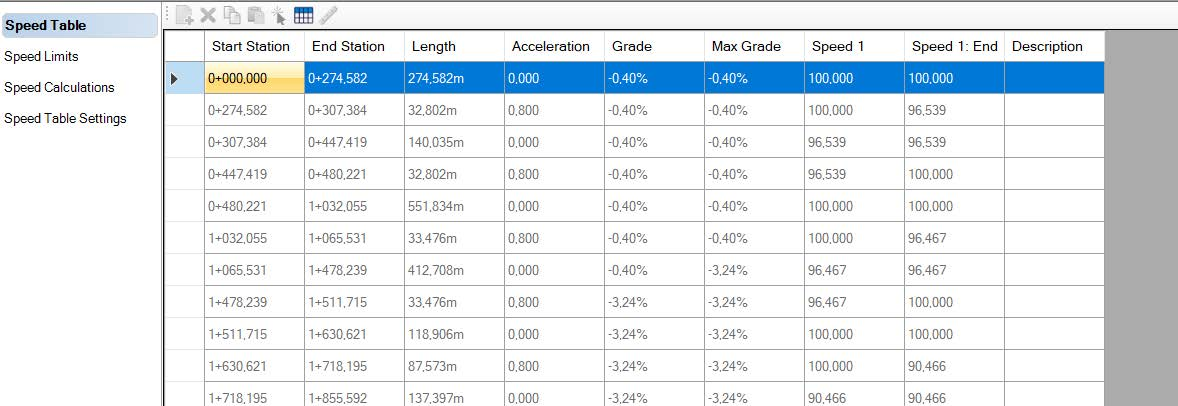
\includegraphics[width=\linewidth]{Figures/Speed Table}
	\captionof{figure}{Speed Table, Verifica delle velocità}
    \label{fig:Speed Table}
\end{figure}

Possiamo calcolare e verificare anche le visibilità attraverso il comando Terrain/Sight Visibility :

\begin{figure}[H]
	\centering
	\includegraphics[width=\linewidth]{Figures/Visibilità}
	\captionof{figure}{Visibilità}
    \label{fig:Visibilità}
\end{figure}